\chapter{Řešení optimalizační úlohy}\label{chap:reseniOptUloh}

V této kapitole vyzkoušíme různé metody, které můžeme pro nalezení optimálního plánu pohotovostní služby použít.

\section{Dynamické programování}\label{kap:dynamicProgram}

\textit{Dynamické programování} je technika řešení problému, která si průběžně ukládá řešení menších podúloh a pomocí rekurzivního vztahu menší podúlohy s větší,
definovaného \textit{Bellmanovou rovností}, řeší větší podúlohy efektivněji, až po vyřešení původní úlohy. 
Průběžnému ukládání výsledků podúloh se říká \textit{memoizace}.
Díky této memoizaci dynamické programování neprohledává prostor řešení duplicitně, a tak je často velmi efektivní metodou pro řešení optimalizačních úloh (\citet{dynamic}).
Triviálním příkladem využití dynamického programování je výpočet $n$-tého \textit{Fibbonaciho čísla}. (\citet{mares}, kap. 12).
\\
\\
Pro nás zajímavějším příkladem využití dynamického programování je řešení úlohy kombinatorické optimalizace \textit{Problému batohu}.

\begin{definice}[Problém batohu]
  Nechť $n$ počet předmětů, které chceme vložit do batohu s kapacitou $c$.
  Každý předmět $i$ má výdělek $p_i$ a váhu $w_i$. Problém batohu pak je,

  \begin{alignat*}{2}
    &\normalfont \text{maximalizuj} \hspace{30pt} &z = \sum_{i=1}^n p_i x_i \\
    \\
    &\normalfont \text{splňující} \hspace{30pt} &\sum_{i = 1}^{n} w_i x_i \leq c,
  \end{alignat*}
  \\
  kde $x_i = 1$, pokud předmět $i$ je v batohu, jinak $0$.
  \\
\end{definice}

Existuje $2^n$ možností, které předměty vložíme do batohu. Naivní řešení prohledání všech možností tak běží v čase $\mathcal{O} (2^n)$.
Avšak pomocí dynamického programování lze vyřešit problém batohu v \textit{pseudopolynomiálním} čase $\mathcal{O}(nc)$,
což pro velká $n$ a konstatní $c$ je až exponenciálním zlepšením.
\\
\\
Bellmanovy rovnice vyjadřující rekurzivní vztahy vypadají následovně,

\begin{definice}[Rekurzivní vztah pro problém batohu]\label{rov:KPrekurz}
  \begin{align*}
    m_{i, c'} &= m_{i - 1, c'} \text{ pokud } w_i > c', \\
    m_{i, c'} &= \max (m_{i - 1, c'}, m_{i - 1, c' - w_i} + p_i) \text{ pokud } w_i \leq c',
  \end{align*}
  \\
  pro $0 \leq c' \leq c$ aktuální uvažovaná kapacita batohu.
\end{definice}

Rekurzivní vztah \ref{rov:KPrekurz} nám pouze říká, že ze znalostí optimálního výběru předmětů podpbroblému $m_{i-1, c' - w_i}$ a podproblému $m_{i - 1, c'}$,
umíme v konstantím čase zjistit optimální výběr předmětů pro aktuální problém $c'$, tedy $m_{i, c'}$.
Buď předmět $i$ použijeme při výběru, a tak aktuální optimální výběr je roven $m_{i - 1, c' - w_i} + p_i$,
nebo předmět při výběru nepoužijeme, takže aktuální optimální výběr je optimální výběr podproblému, $m_{i - 1, c'}$. 

\begin{algorithm}
  \begin{algorithmic}[1]
  \Function{KnapsackProblem}{$n$, $c$, $p_i$, $w_i$, $1 \leq i \leq n$}
    \State $m_{i, j}$ \gets 0, $0 \leq i \leq n$, $0 \leq j \leq c$
    \For{$1 \leq i \leq n$}
      \For{$1 \leq j \leq c$}
        \If{$w_i > j$}
          \State $m_{i, j}$ \gets $m_{i - 1, j}$
        \Else
          \State $m_{i, j}$ \gets $\max$ ($m_{i - 1, j}$, $m_{i - 1, j - w_i} + p_i$)
        \EndIf
      \EndFor
    \EndFor
    \State \Return $m_{n,c}$
  \EndFunction
  \end{algorithmic}
  \caption{}
  \label{KP}
\end{algorithm}

Algoritmus \ref{KP} vrací sumu hodnot optimálních předmětů přidaných do batohu.
Jaké konkrétní předměty přispěly do sumy lze snado zjistit zpětným následováním rekurzivního vztahu \ref{rov:KPrekurz}.
\\
\\
Rádi bychom našli nějaký rekurzivní vztah v problému hledání optimálního plánu.

Avšak ukáže se, že takový rekurzivní vztah neexistuje.
Ze znalosti optimálního plánu podproblému obecně nelze zjistit optimální plán aktuálního problému.
Ukážeme si na konkrétním příkladu. 

\begin{figure}[h]
\includegraphics[width=0.4 \textwidth]{img/bak_dp_protipriklad1}
\caption{Tři výjezdové stanice, hnědé kruhy a tři modré incidenty, modré kruhy. Incidenty jsou očíslované podle času nastání.}
\label{obr:protipriklad1}
\end{figure}

\clearpage

Nechť incidenty $i_1$, $i_2$, $i_3$ podle obrázku \ref{obr:protipriklad1} v časech nastání $t_1$, $t_2$, $t_3$.
Řekněme, že optimální plán pohotovostní služby $p_1$ pro tento případ je alokace tří týmů záchranářů se směnami $d_1$, $d_2$, $d_3$ a záchranných vozidel, každý na jednu stanici.
Tým záchranářů $Z_A, p_Z(Z_A) = A$, odbaví incident $i_1$, $Z_B$ odbaví $i_3$ a $Z_C$ odbaví $i_2$.
Další incident, který nastane je $i_4$.

\begin{figure}[h]
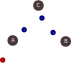
\includegraphics[width=0.4 \textwidth]{img/bak_dp_protipriklad2}
\caption{Nastal nový incident.}
\label{obr:protipriklad2}
\end{figure}


